\chapter{OpenGL for Embedded Systems}
\todo{Der skulle gerne stå et sted i rapporten før det her afsnit hvad OpenGL ES står for. (Acronym)}
OpenGL is a 2D and 3D graphics API. It is cross-platform API that specifies a standard for 3D graphics processing hardware. Android have support for \ac{opengles} up to version $2.0$. Android $1.0$ and later versions have support for \ac{opengles} $1.0$ and $1.1$ specifications. Android $2.2$ added support for \ac{opengles} $2.0$. \citep{androidopengl, khronosopengl, khronosopengles}

\subsection*{Choice of \ac{opengles} Version}
When using \ac{opengles} on the Android platform, the default \ac{opengles} version is $1.x$. If you want to use version $2.0$ you need to explicitly write that you are using it. Version $2.0$ should have better performance and more possibilities than the older version, but the Android developers guide says:
\begin{quote}
\textit{"Developers who are new to OpenGL may find coding for \ac{opengles} 1.0/1.1 faster and more convenient."} \citep{androidopengl}
\end{quote}
Since we are newbies to OpenGL we have chosen version $1.x$. One big difference between $1.x$ and $2.0$ is that you have to write your own shaders in versions $2.0$, this allows for easier effects customisation. The Train game does not really require much special effects other than simple drawing of textures.

\section{Design}
Firstly \autoref{fig:terminology} shows how we represent abstract class names and how we denote public or private attributes and methods. A minus denotes a private attribute/method, and a plus denotes a public attribute/method. Italic class names are abstract classes.
\begin{figure}[H]
\centering
\includegraphics[page=4,width=0.7\linewidth]{img/opengl.pdf}
\caption{The way we make UML described in a figure.}
\label{fig:terminology}
\end{figure}

\subsection{Renderable Classes}

Thinking about what the game is suppose to do we came up with the different objects we need to be able to render. \autoref{fig:renderables} shows a simplified version of the different objects/classes that can be rendered. We needed to draw texture at different positions on the screen and we needed to be able to move texture around on the screen. This is the general idea and based on this, the following classes was created.

\begin{figure}[H]
\centering
\includegraphics[page=2,width=1\linewidth]{img/opengl.pdf}%0.1 margin
\caption{Class diagram of the objects that can be rendered.}
\label{fig:renderables}
\end{figure}

\begin{description}
\item[Coordination/Renderable:] In order to move objects around we have the abstract super class \lstinline|Coordination| which defines the methods to move. The abstract class \lstinline|Renderable| specify that objects that should be rendered on the screen must implement the abstract methods: \lstinline|draw|, \lstinline|getWidth|, and \lstinline|getHeight|. If some \lstinline|Renderable| object should be drawn more than one place, then instead of making two identical \lstinline|Renderable| objects with different coordinates, we have a list of coordinates in \lstinline|Coordination|. The \lstinline|move| method will then move all the coordinates by the specified amount. It was also a possibility to move only one specific coordinate by the specified amount, but this last scenario was never needed.

\item[RenderableMatrix:] Since almost everything is moved relative to the train's speed we needed some kind of grouping of \lstinline|Renderable| objects, that were moved together. This is what \lstinline|RenderableMatrix| handles. It is possible to add other \lstinline|Renderable| objects to the \lstinline|RenderableMatrix|, this means that it is also possible to add matrices to matrices. The \lstinline|addRenderMatrixItem| method also have a color as parameter to use when drawing the \lstinline|Renderable|, this parameter is not shown on the figure to reduce the size of it. When calling \lstinline|draw| on the matrix, it iterates through all \lstinline|matrixItems| and calls draw on them. The color parameter to the matrix is ignored, and instead uses the color specified for each matrix item.

The \lstinline|RenderableMatrix| must also implement the abstract methods \lstinline|getWidth| and \lstinline|getHeight|. The width is calculated by the difference between the lowest x-coordinate to the greatest x-coordinate, and the same goes for the height with the y-coodinate instead. This feature was used at the time when this was designed, but has later become unnecessary.

The \lstinline|RenderableMatrix| is made with a new OpenGL matrix, this will be explained in more detail in \secref{sec:gamerendering}.

\item[Shape:] Everything that takes the form of a shape e.g. a square or a triangle, must inherit from the abstract class \lstinline|Shape|. All shapes consists of an array of vertices. Since we need wheels to rotate on the train, \lstinline|Shape| implements a method to rotate the \lstinline|Shape| around its center.

\item[Square:] The \lstinline|Square| is initialised with a size in the constructor, and then vertices are created according to the specified size. The color in the \lstinline|draw| method's parameter specify the color of the square.

\item[GradientSquare:] This is similar to the \lstinline|Square|, instead this square is initialised with two colors to create either a horizontal or a vertical color gradient between the two colors.

\item[Texture:] This is the most important and most used class when creating our game. Since all pictures/images are 'square', then it is obvious why the texture inherits from \lstinline|Square|. There are a lot different ways to implement texture, and the different ways will not be discussed. This class must at some point load a resource pointer to a texture pointer. The loaded texture will always stretch to the size of the \lstinline|Square| that it is drawn upon. The \lstinline|Texture| class also implements ways to keep the original aspect ratio of the texture, although not shown in the figure, the \lstinline|loadTexture| method also has an aspect ratio option that allows the size of the \lstinline|Square|, containing the texture, to resize based on the size of the texture.

The \lstinline|draw| method must be overridden in order to draw the loaded texture. In this case it is possible to change the color that the \lstinline|Texture| is drawn with. No matter what color the original \lstinline|Texture| is, a color filter can be put on top of that on each call of the draw method.

\item[Text:] Adds the possibility to draw text. \lstinline|loadText| generates a bitmap with the specified text to use as texture. This is an easy way to draw text, but if you need to draw text that changes all the time, then \lstinline|loadText| is a slow way to do it. Fortunately we only need to load one time for each \lstinline|Text| object.

\item[GlPictogram:] Adds the possibility to draw a pictogram. \lstinline|loadPictogram| generates a bitmap of the pictogram image, and then uses it as the texture for the object. To draw the pictogram text, a \lstinline|Text| object is used.\todo{Skriv i weekly notes hvorfor vi også har GlPictogram klassen som en Renderable i stedet for kun View}
\end{description}

\subsection{Texture Power-of-two Support}
Some \ac{opengles} devices does not support texture with a \ac{npot} size, they only accept texture with a \ac{pot} size. Android developers reference states that you should perform a check whether the current context supports \ac{npot}. \citep{glutils}

It is hard to find a proper reference to why \ac{npot} is not supported. A lot different developers says it is because you get an increase of performance when using \ac{pot}, and at the time when the first version of OpenGL was created, the hardware needed this extra performance. Later hardware only gained an insignificant increase of performance so they allowed \ac{npot}. Some Embedded System using \ac{opengles} still gain a significant increase in performance, and this is why some devices require texture to be \ac{pot}.\todo{Er det i orden at sige vi ikke har en reference? Skal vi bare tilføje referencer til upålidelige kilder?}

Instead of performing a check to see whether the current context supports \ac{npot}, we choose to always use \ac{pot}. Even if it is not neccesary it will still give a small performance increase. The way we achieve this is to still use texture with a \ac{npot} size, convert the texture to \ac{pot} size, and then stretch it relative to the change in size.
\begin{figure}[H]
\begin{minipage}[b]{0.5\columnwidth}
\centering
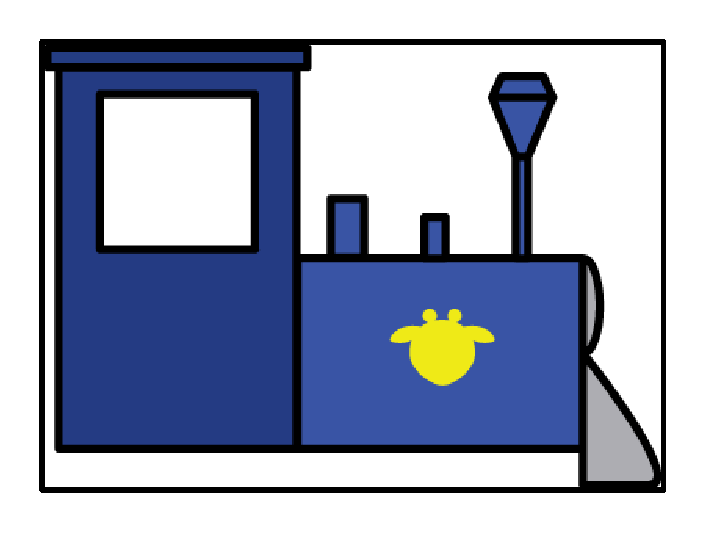
\includegraphics[page=1,width=0.8\columnwidth]{img/powerOfTwo.pdf}
\caption{The \ac{npot} train texture inside the \lstinline|Square| container.\label{fig:train}}
\end{minipage}
\hspace{0.5cm}
\begin{minipage}[b]{0.5\columnwidth}
\centering
\includegraphics[page=2,width=0.8\columnwidth]{img/powerOfTwo.pdf}
\caption{The \ac{pot} train texture.\label{fig:trainpot}}
\end{minipage}
\end{figure}
\autoref{fig:train} shows the train texture inside the \lstinline|Square| container. The black line illustrates the \lstinline|Square|, this is shown for the sake of the example and it is of course not shown in the actual application. The texture has a size of $396 \times 284$ pixels, and need to be converted to a \ac{npot} size.

\autoref{fig:trainpot} shows the train texture with alpha channels to the right and below the texture to obtain a \ac{pot} texture with the size of $512 \times 512$ pixels.
\begin{figure}[H]
\begin{minipage}[b]{0.5\columnwidth}
\centering
\includegraphics[page=3,width=0.8\columnwidth]{img/powerOfTwo.pdf}
\caption{The \ac{pot} train texture inside the \lstinline|Square| container.\label{fig:trainneedcrop}}
\end{minipage}
\hspace{0.5cm}
\begin{minipage}[b]{0.5\columnwidth}
\centering
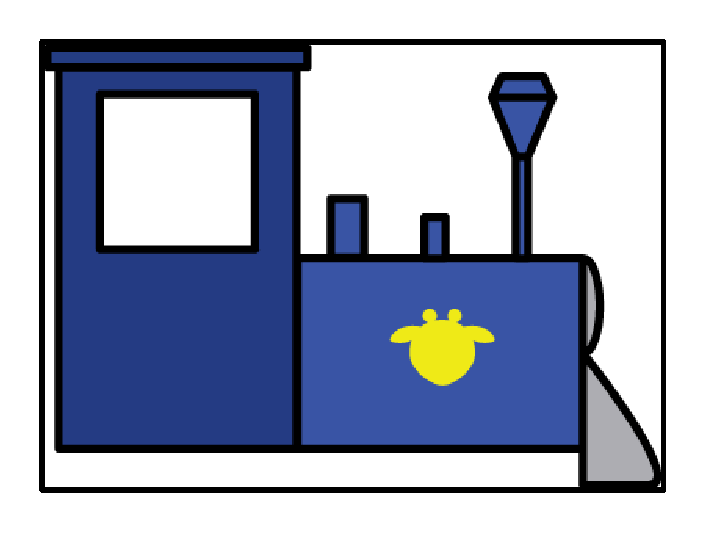
\includegraphics[page=1,width=0.8\columnwidth]{img/powerOfTwo.pdf}
\caption{The \ac{pot} train texture after cropping.\label{fig:trainresult}}
\end{minipage}
\end{figure}
When we take the new \ac{pot} sized texture and insert it into the \lstinline|Square| the texture will still clamp to the edges. \autoref{fig:trainneedcrop} shows the clamped train texture.

We need to adjust the texture vertices in order to fit the \ac{pot} texture inside the \lstinline|Square|. We stretch the texture relative to the change in size from \ac{npot} to \ac{pot}. You could also say that the extra alpha channels are cropped away. \autoref{fig:trainresult} shows the result of the texture conversion from \ac{npot} to \ac{pot}.\todo{Skal \autoref{fig:trainresult} også indeholde de stiplet linjer udenfor firkant-rammen?}

\subsection{Game Rendering}\label{sec:gamerendering}

\begin{figure}[H]
\centering
\includegraphics[page=3,width=1\linewidth]{img/opengl.pdf}%0.1 margin
\caption{Class diagram of the objects involved with drawing the game.}
\label{fig:game}
\end{figure}

\begin{description}
\item[GlRenderer] 
\item[GameDrawer] 
\item[GameDrawable] 
\item[GameData] 
\end{description}

\section{Implementation}
\todo{Describes the implementation of OpenGL}
